\documentclass[aspectratio=169]{beamer}

\usepackage[utf8]{inputenc}
%\usepackage{latexsym}
\usepackage{graphicx}
\usepackage{mathptmx}
\usepackage{amsmath}
%\usepackage{amsfonts}
\usepackage{amssymb}
\usepackage{amsbsy}
\usepackage{amsthm}
\usepackage{algorithmic}

% Get checkmark logo
\usepackage{pifont}
\newcommand{\cmark}{\ding{51}}
\newcommand{\xmark}{\ding{55}}
% Get \lee and \gee commands
\newcommand{\lee}{\leqq}
\newcommand{\gee}{\geqq}

\usepackage[english]{babel}
\usepackage[utf8]{inputenc}

% AMSLaTeX packages
\usepackage{amsthm}
\usepackage{amsmath}
\usepackage{amsfonts}
\usepackage[algoruled]{algorithm2e}

\usetheme{default}
\useoutertheme{default}
% we want to use images
\usepackage{graphicx}
\usepackage{movie15}
\usepackage{hyperref}

% table relates packages
\usepackage{booktabs}
\usepackage{multirow}
% pick a font
\usepackage{palatino}           
% \usepackage{times}
\usepackage{tikz}
\usetikzlibrary[positioning,arrows,decorations.pathmorphing,backgrounds,fit,calc]
% \AtBeginSection[]  % "Beamer, do the following at the start of every section"
% {
%   \begin{frame}<beamer> 
%     \frametitle{Outline} % make a frame titled "Outline"
%     \tableofcontents[currentsection]  % show TOC and highlight current section
%   \end{frame}                    
% }

% \AtBeginSubsection[]
% {
%   \begin{frame}
%     \frametitle{Outline}
%     \tableofcontents[currentsection,currentsubsection]
%   \end{frame}
% }

\AtBeginSection[]
{
   \begin{frame}
       \frametitle{Outline}
       \tableofcontents[currentsection]
   \end{frame}
}

\newcommand{\ebox}[1][1em]{\framebox[#1]{\phantom{M}}}

\setlength\arraycolsep{1.4pt}% some length

%gets rid of navigation symbols
\setbeamertemplate{navigation symbols}{}

%gets rid of bottom navigation bars
\setbeamertemplate{footline}[page number]{}
\setbeamertemplate{headline}{}


\usebackgroundtemplate{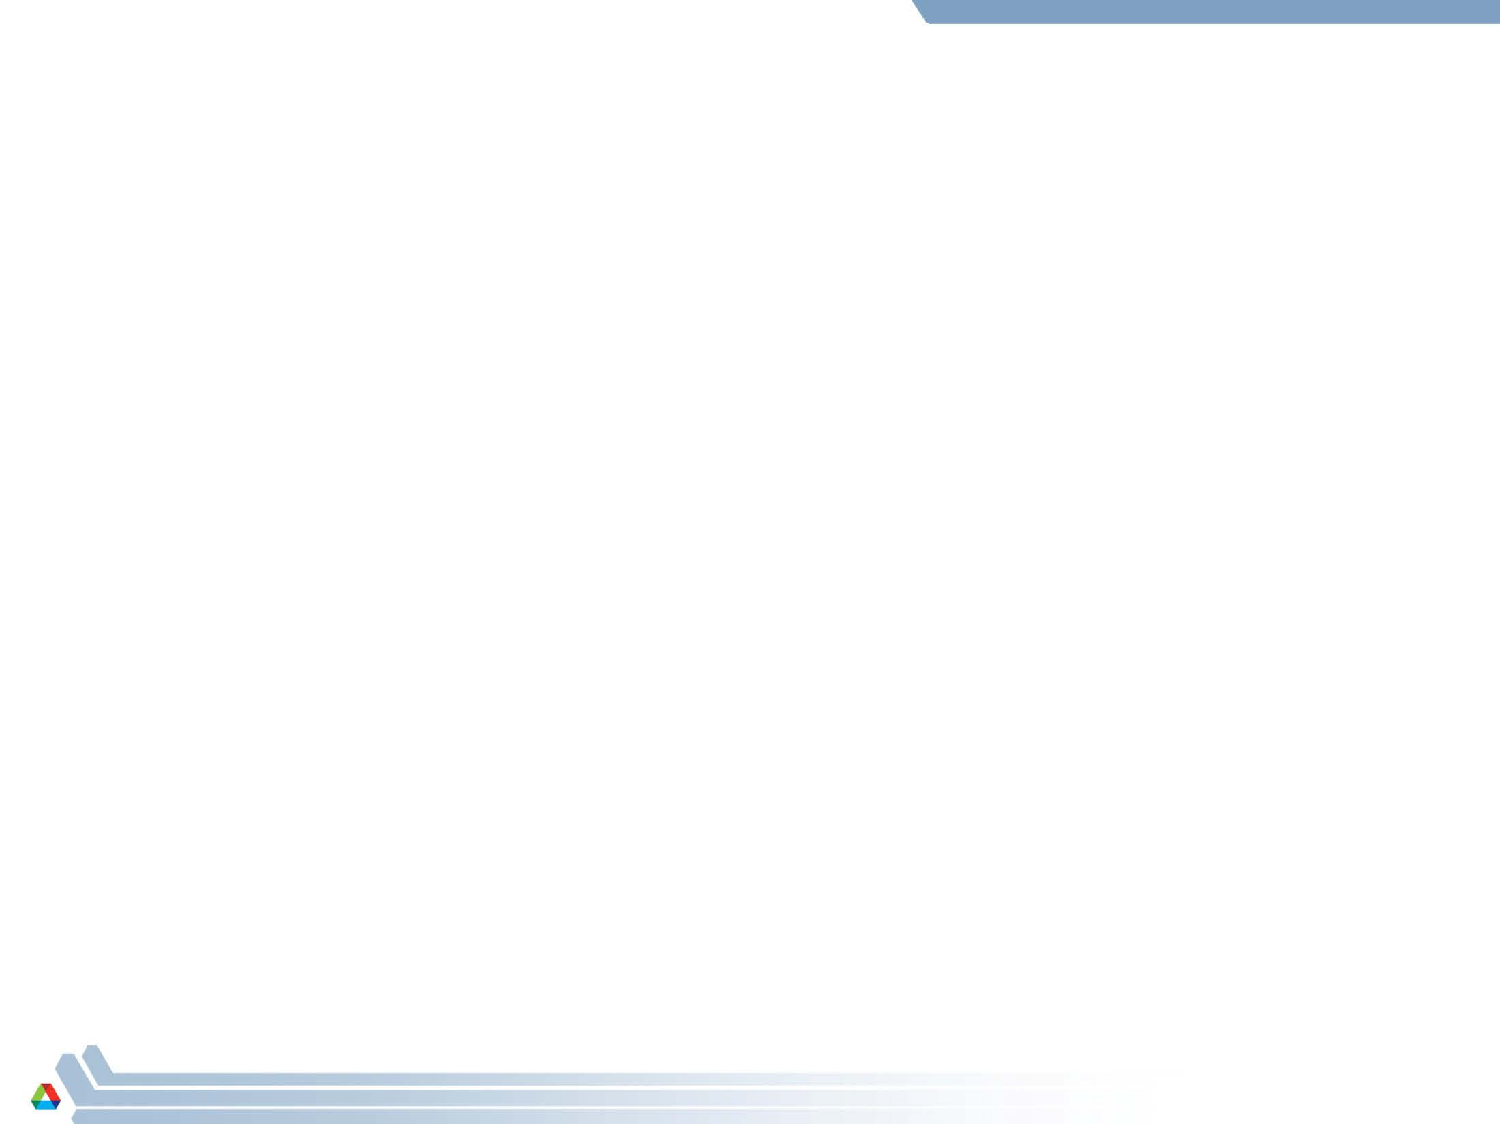
\includegraphics[width=\paperwidth]{../templates/NormalANLBlue}}
% Title Information
\title{Multivariate interpolation and spatial graphs by computing sparse
subsets of the Delaunay triangulation}
\author{Tyler Chang}
\date{LANS Seminar Series\\
July 12, 2023}
\institute{Argonne National Laboratory}

\begin{document}

\setbeamertemplate{footline}{}
{
\usebackgroundtemplate{
\includegraphics[width=\paperwidth]{../templates/TitleANLBlue}}
\frame{\titlepage}
}

\setbeamertemplate{footline}[page number]{}

% FRAME: overview
\begin{frame}
  \frametitle{Outlines}
  \tableofcontents
\end{frame}

\section{Delaunay Interpolation}

% What is Delaunay triangulation
\subsection{Introduction and Motivation}
\begin{frame}{About Delaunay Triangulations}
\begin{itemize}
\item The {\it Delaunay triangulation} is an unstructured simplicial mesh
defined by an arbitrary vertex set
$P = \{x^{(1)}, \ldots, x^{(n)}\} \subset \mathbb{R}^d$
\item The defining property of the Delaunay triangulation $DT(P)$ is that
for every simplex $S \in DT(P)$, the circumball $B^{(S)}$
must have empty intersection with $P$:
$B^{(S)} \cap P = \emptyset$.
\end{itemize}
\begin{center}
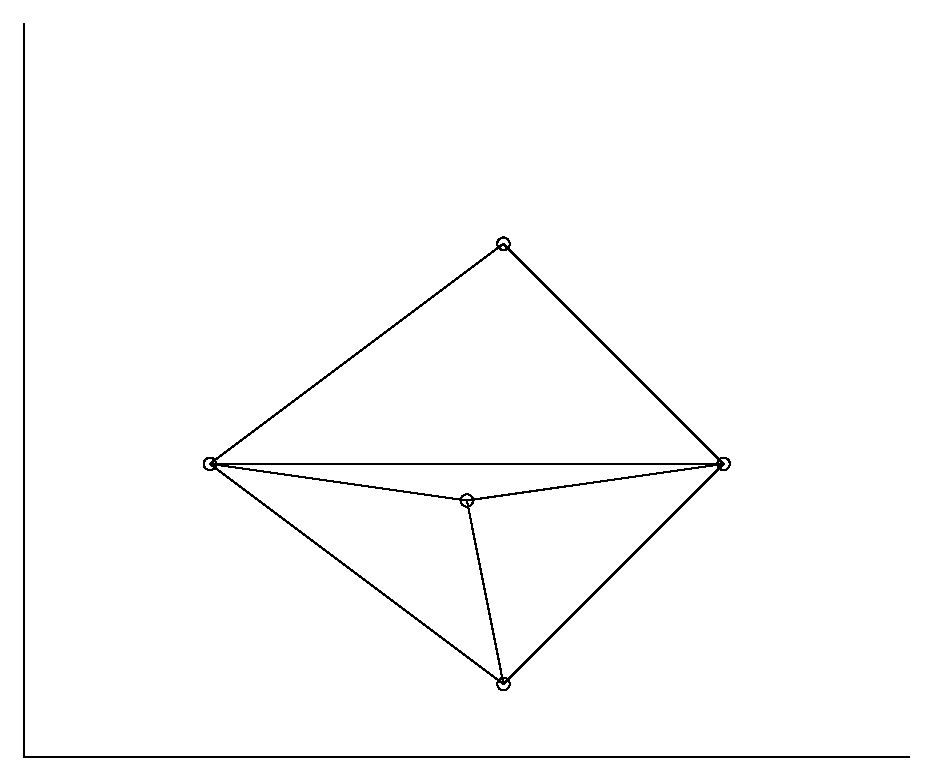
\includegraphics[width=0.25\textwidth]{../img/delaunay_old/triangleplane.eps}
\hskip 4pt{\color{red} \xmark}
$\qquad\qquad$
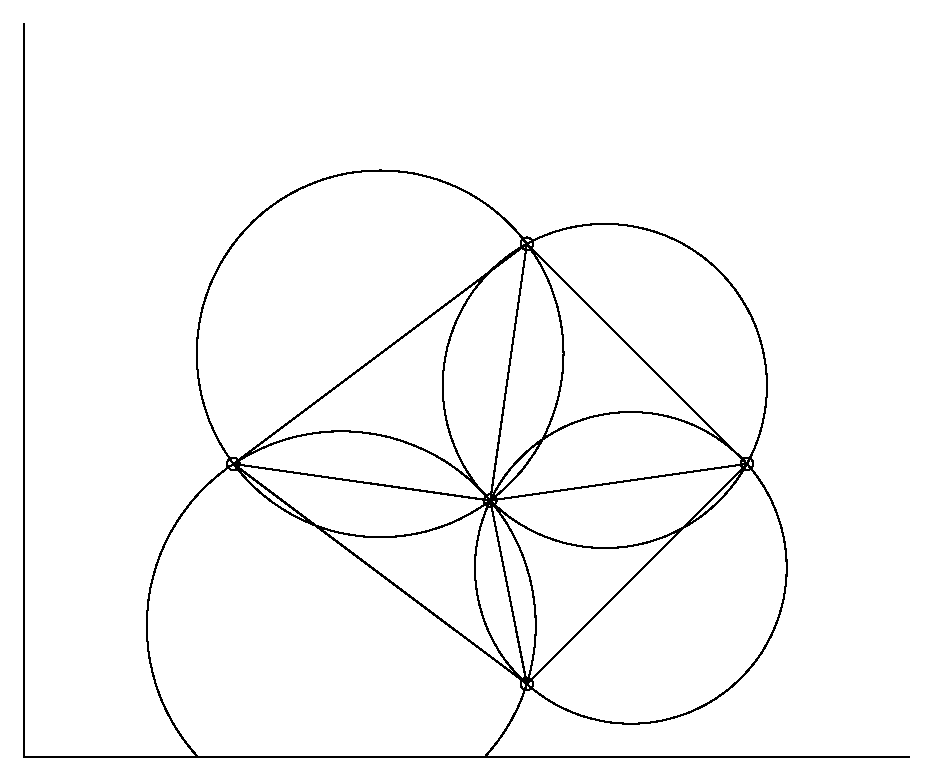
\includegraphics[width=0.25\textwidth]{../img/delaunay_old/delaunayplane.eps}
\hskip 4pt{\color{green} \cmark}
\end{center}
\begin{itemize}
\item $DT(P)$ exists and is unique when $P$ is in {\it general position}.
\end{itemize}
\end{frame}

% Brief applications of Delaunay
\begin{frame}{Delaunay Interpolation}
\begin{columns}
\begin{column}{.58\textwidth}
Let $y \in S \in DT(P)$.
$S$ has vertex set $\{s^{(1)}, \ldots, s^{(d+1)}\}$ and there exist
convex weights $\{w_1, \ldots, w_{d+1}\}$ such that
$y = \sum_{i=1}^{d+1} w_i s^{(i)}$.
$$
{\hat F}_{DT}(y) = \sum_{i=1}^{d+1} w_i F(s^{(i)}).
$$
\end{column}
\begin{column}{.38\textwidth}
\hbox{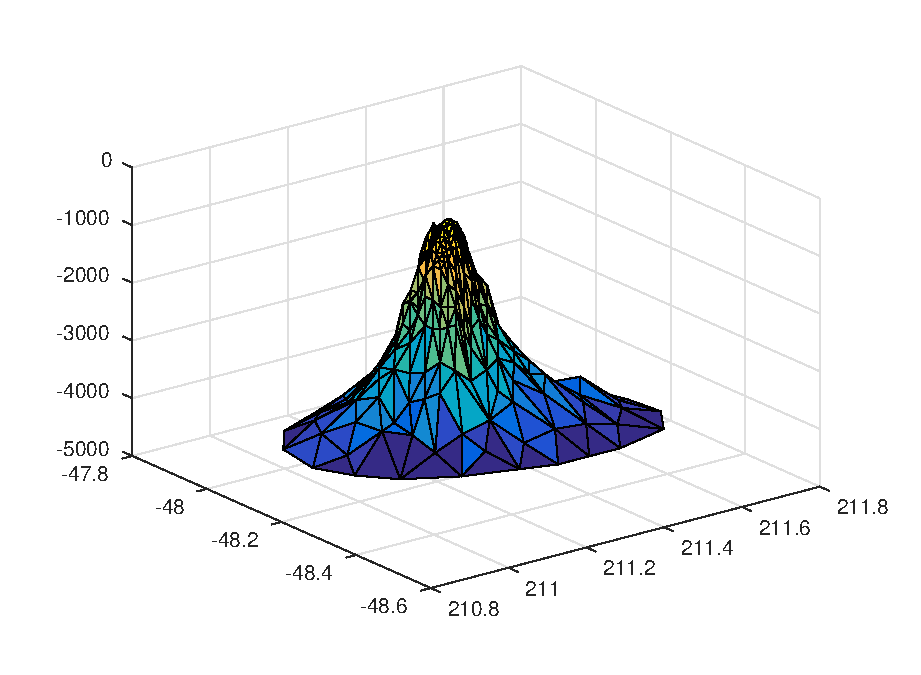
\includegraphics[width=\textwidth]{../img/delaunay_old/seamount.eps}}
\end{column}
\end{columns}
\medskip
Advantages in data science/ML settings
\begin{itemize}
\item Interpolates data (when that is a desirable property)
\item Like a feed-forward fully-connected ReLU net, this is a piecewise linear
model.
But this model is provably considered ``optimal'' (in a sense) for
interpolation w.r.t. other piecewise linear models.
\item Can be used to interpolate functional response variables, e.g., PDFs.
\end{itemize}
\end{frame}
% Some properties of Delaunay that we will need
\begin{frame}{Scalability Issues}
\begin{itemize}
\item Oweing to Klee, the size of the Delaunay triangulation is
$$
\mathcal{O}\left(n^{\lceil d/2 \rceil}\right)
$$
\begin{itemize}
\item For $d > 4$, this is expensive!
\item For $d > 8$, this is not scalable!
\end{itemize}
\end{itemize}
\pause
{\textbf{Observation:}
For interpolation at a single point $y$, we only need the
vertices ($\{s^{(1)}, \ldots, s^{(d+1)}\}$) of $S \in DT(P)$
such that $y\in S$}
$$
{\hat F}_{DT}(y) = \sum_{i=1}^{d+1} w_i\text{~}F(s^{(i)}).
$$
\medskip
\pause
{\textbf{Question:} Can we find $S$ containing $y$ in polynomial time?}
\end{frame}

% Algorithm description
\subsection{Algorithm Description}
% Algorithm for computing the Delaunay interpolant
\begin{frame}{Algorithm outline}
Algorithm to locate Delaunay simplex containing $y$:
\begin{itemize}
\item Grow an initial Delaunay simplex (greedy algorithm) that is
``nearby'' to $y$
\item ``Flip'' accross facets from which $y$ is visible to a new Delaunay
simplex (closer to $y$)
\item This ``visibility walk'' converges to $y$ in finite steps
(Edelsbrunner's acyclicity theorem)
\end{itemize}
\vfill
{\tiny \it Chang, Watson, Lux, Li, Xu, Butt, Cameron, and Hong.
``A polynomial time algorithm for multivariate interpolation in arbitrary
dimension via the Delaunay triangulation.''
In Proc. 2018 ACMSE Conf.}
\end{frame}

% First simplex
\begin{frame}{Growing the First Simplex}
$\phi$ is the vertex set for the initial Delaunay simplex:
\begin{itemize}
\item Start with $\phi$ containing just the nearest neighbor to $y$ in
$P$;
\item For all $x \in P \setminus \phi$, compute the radius $r_{min}$ of
the smallest circumball about $\{x\} \cup \phi$ and select the $x^*$
that minimizes $r_{min}$;
\item $\phi \leftarrow \phi \cup \{x^*\}$;
\item Repeat until $|\phi| = d+1$;
\end{itemize}
\begin{lemma}
Let $P$ be in general position, and
let $\Gamma$ be a Delaunay $j$-face with vertices $\phi \subset P$
where $j<d$.
Let $x^* \in P \setminus \phi$
minimize the radius of the smallest $(d-1)$-sphere through the points in
$\phi \cup \{x\}$, over all $x \in P \setminus \phi$.
Then $\Gamma^* = \text{ConvexHull}(\phi \cup \{x^*\})$ is a Delaunay
$(j+1)$-face.
{\bf Proof in Paper.}
\end{lemma}
\end{frame}

% How to flip across an open facet
\begin{frame}{Flipping}
\begin{columns}
\begin{column}{.58\textwidth}
\begin{itemize}
\item Let $\phi$ be the vertices for a facet of a Delaunay simplex;
\item Let $\Gamma$ be the facet with vertices in $\phi$;
\item Let $H$ be the halfspace containing $y$,
w.r.t. the hyperplane containing $\Gamma$
\item Unless $\Gamma$ is a facet of the convex hull, there exists
$x^* \in P \setminus \phi$ such that $\phi \cup \{x^*\}$
is the vertex set for a Delaunay simplex;
\end{itemize}
\end{column}
\begin{column}{.4\textwidth}
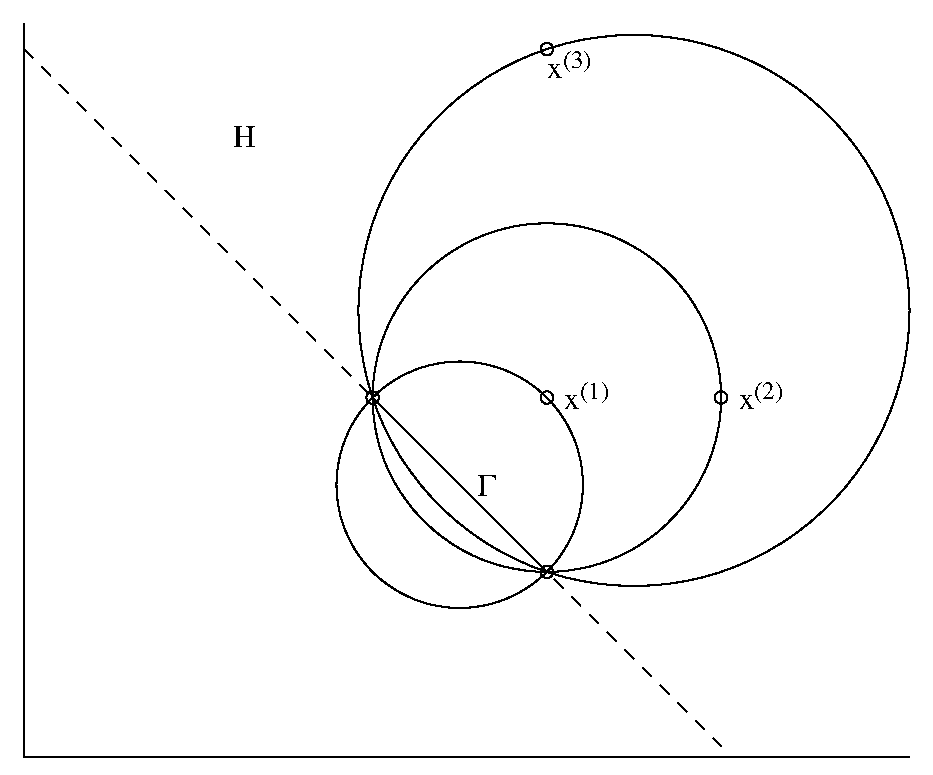
\includegraphics[width=\textwidth]{../img/delaunay_old/circles.eps}
\end{column}
\end{columns}
\medskip
\centerline{\bf Proof in Paper.}
\end{frame}

% The visibility walk
\begin{frame}{Visibility walk}
\begin{columns}
\begin{column}{.48\textwidth}
\begin{itemize}
\item Grow an initial simplex $S^{(0)}$;
\item While $y \not\in S^{(k)}$, generate $S^{(k+1)}$ by flipping
across a facet of $S^{(k)}$ from which $y$ is ``visible'';
\item Terminate when $y\in S^{(k)}$, otherwise, $k \leftarrow k+1$;
\end{itemize}
\end{column}
\begin{column}{.48\textwidth}
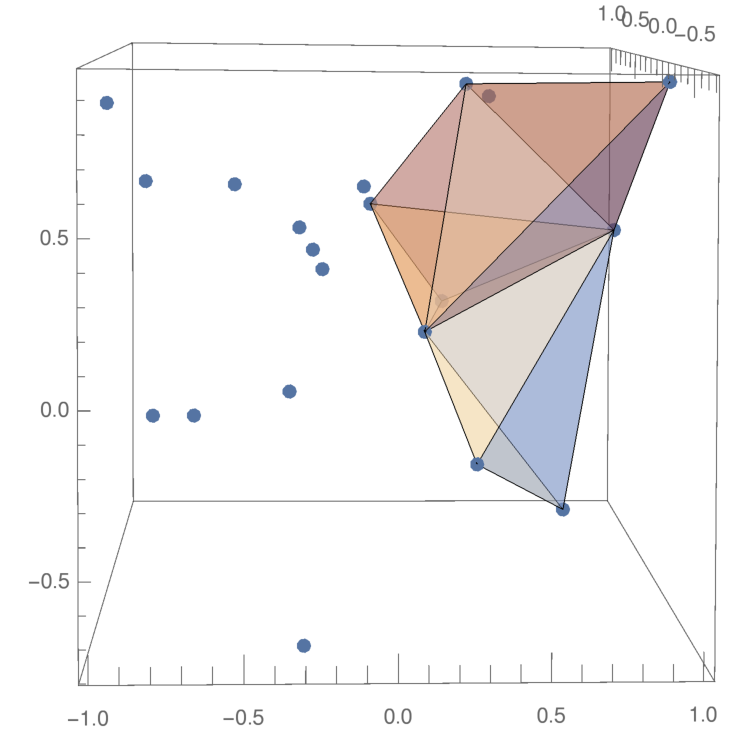
\includegraphics[width=\textwidth]{../img/delaunay_old/DelaunayWalk.pdf}
\end{column}
\end{columns}
\medskip
Converges in finite flips by {\it Edelsbrunner's Acyclicity Theorem}.
\end{frame}

% Complexity
\begin{frame}{Algorithm Complexity}
\begin{itemize}
\item To grow the first simplex:
$\mathcal{O}(n d^3)$ to apply $n$ rank-1 updates to the QR factorization of
$d \times j$ matrix for $j=1,\ldots,d$
\item To compute a flip:
$\mathcal{O}(n d^2)$ to apply $n$ rank-1 updates to the QR factorization of
a $d \times d$ matrix
\item $\ell$ total flips\\
\centerline{\small
\begin{tabular}{l|cccc}
  & $n=2K$ & $n=8K$ & $n=16K$ & $n=32K$\\
\hline
$d=2$  & 3.05 & 2.90 & 3.25 & 3.10\\
$d=8$  & 23.75 & 24.75 & 24.30 & 23.10\\
$d=32$ & 95.25 & 125.60 & 131.85 & 150.10\\
$d=64$ & 171.95 & 221.85 & 248.35 & 280.60\\
\end{tabular}}
\end{itemize}
\medskip
\pause
{\bf Overall complexity:} $\mathcal{O}(nd^2 \ell)$\\
\medskip
\pause
{\bf Unresolved question:} $\ell \approx d$? $\ell$ independent of $n$?
\end{frame}

% Linear programming
\begin{frame}{Linear programming interpretation}
$$
{\tilde A} = \left[ \begin{matrix}
(-x^{(1)})^T & 1 \cr
(-x^{(2)})^T & 1 \cr
\vdots & \vdots \cr
(-x^{(n)})^T & 1 \cr
\end{matrix}\right]\text{, }
{\tilde b} = \left[ \begin{matrix}
\| x^{(1)} \|_2^2 \cr
\| x^{(2)} \|_2^2 \cr
\vdots \cr
\| x^{(n)} \|_2^2 \cr
\end{matrix}\right]\text{, and }
{\tilde c} = \left[ \begin{matrix}
-y \cr
1 \cr
\end{matrix}\right].
$$
\pause
$\displaystyle \hbox{\bf Primal prob: }
\max_{\tilde u} {\tilde c}^T {\tilde u}
\hbox{ such that }
{\tilde A}{\tilde u} \leq {\tilde b}, {\tilde u}\hbox{ free}.$\\
{\bf Ext pts:}
${\tilde u} = (-2\hbox{circumcenter}, \hbox{circumradius}^2 - \|\hbox{circumcenter}\|_2^2)$\\
\medskip
\pause
$\displaystyle \hbox{\bf Dual prob: }
\min_{\tilde v} {\tilde b}^T {\tilde v}
\hbox{ such that }
{\tilde A}^T{\tilde v} = {\tilde c}, {\tilde v}\geq 0.$\\
{\bf Ext pts:}
$\Rightarrow$ ${\tilde v}$ are convex weights for $y$\\
\medskip
\pause
Primal + dual feasible $\Rightarrow$ Delaunay simplex containing $y$\\
\medskip
\pause
{\bf LP basic solution in polynomial time is an open problem!}
\end{frame}

%% Extrapolation
%\begin{frame}{Extrapolation}
%What about extrapolation?
%\begin{itemize}
%\item Project $y$ on to the convex hull of $P$
%\item Interpolate the projection (if the residual is small)
%\item Note: projection is a quadratic program (more expensive than an LP)
%\end{itemize}
%Let $E$ be a $d\times n$ matrix whose columns are points in $P$, and let
%$z$ be an extrapolation point (outside convex hull of $P$).
%$$
%\xi^* = \arg\min_{\xi\in\mathbb{R}^n} \|E\xi - z\| \quad\hbox{subject to}\quad
%\xi \ge 0 \quad\hbox{and}\quad \sum_{i=1}^n \xi_i = 1.
%$$
%Projection: ${\hat z} = E\xi^*$
%\end{frame}

% Implementation description
\subsection{Implementation}
% DELAUNAYSPARSE
\begin{frame}{DELAUNAYSPARSE Package}
Standalone software package {\tt DELAUNAYSPARSE}:
\begin{columns}
\begin{column}{.5\textwidth}
\begin{itemize}
\item Robust against degeneracy
\item Runs in $\mathcal{O}(m n d^2 \ell)$ time
\end{itemize}
\end{column}
\begin{column}{.5\textwidth}
\begin{itemize}
\item Parallel and serial implementations
\end{itemize}
\end{column}
\end{columns}
\begin{columns}
\begin{column}{.15\textwidth}
Runtime (secs) for interpolating a single point ($m=1$) with $n$ pts
in $\mathbb{R}^d$
\end{column}
\begin{column}{.8\textwidth}
{\small
\begin{center}
\begin{tabular}{c|rrrrr}
& & & $d\quad$ & & \\
$n$ & $2\quad$ & $8\quad$ & $32\quad$ & $64\quad$ & $128\quad$ \\
\hline
250    & 0.005  & 0.013   & 0.150   & 3.404    & 27.078   \\
500    & 0.021  & 0.042   & 0.325   & 6.479    & 59.511   \\
1000   & 0.083  & 0.152   & 0.791   & 14.020   & 124.320  \\
2000   & 0.344  & 0.583   & 2.230   & 28.984   & 242.066  \\
4000   & 1.314  & 2.284   & 7.165   & 62.494   & 502.620  \\
8000   & 5.580  & 9.027   & 26.210  & 151.177  & 905.711  \\
16,000 & 22.086 & 35.725  & 109.448 & 386.596  & 2190.362 \\
32,000 & 82.915 & 145.115 & 421.934 & 1097.060 & 5024.675 \\
\end{tabular}
\end{center}
}
\end{column}
\end{columns}
\vfill
{\tiny \it Chang, Watson, Lux, Butt, Cameron, and Hong. 2020.
Algorithm 1012: DELAUNAYSPARSE: Interpolation via a sparse subset of the
Delaunay triangulation in medium to high dimensions.
ACM Trans.\ Math.\ Softw.\ 46(4).}
\end{frame}

% Parallel implementation
\begin{frame}{Parallel implementation}
\textbf{Distributed memory:} Run
the serial algorithm on small batches of interpolation pts\\
\medskip
{\bf Shared memory:} Multiple levels
\begin{itemize}
\item Level 1: loop over multiple interpolation points (like distributed case)
\item Level 2: loop(s) over data points -- results in additional work;
preferrable only when $m$ is small and $n$ is large
\end{itemize}
\begin{columns}
\begin{column}{.5\textwidth}
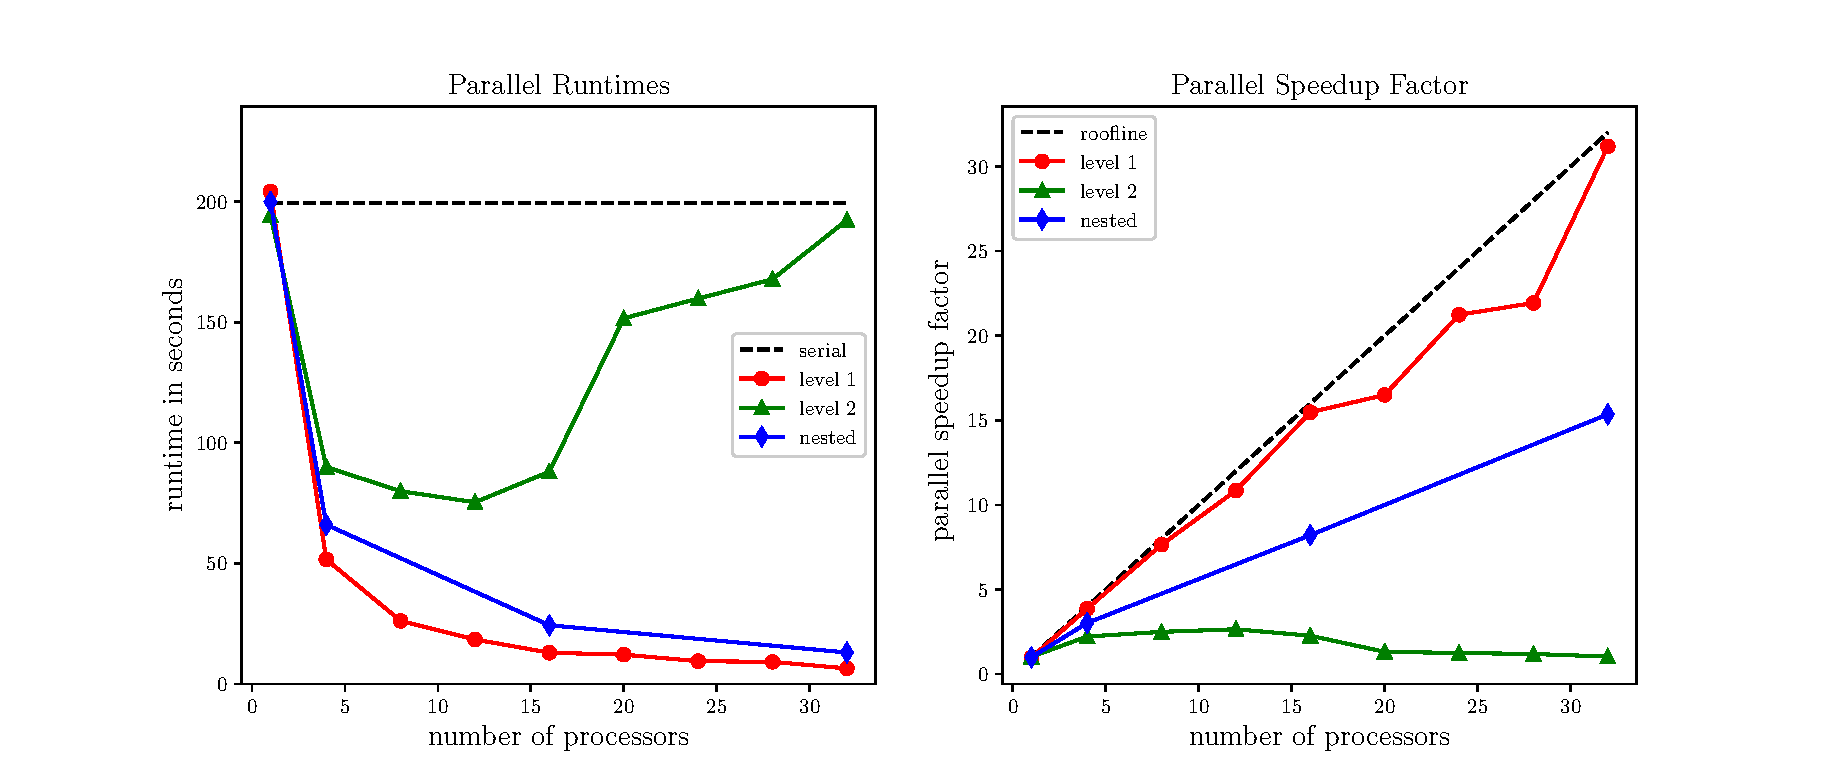
\includegraphics[width=\textwidth]{../img/delaunay_old/parallelBigD.eps}
\begin{center}$d=50\text{, }n=500\text{, }m=64$\end{center}
\end{column}
\begin{column}{.5\textwidth}
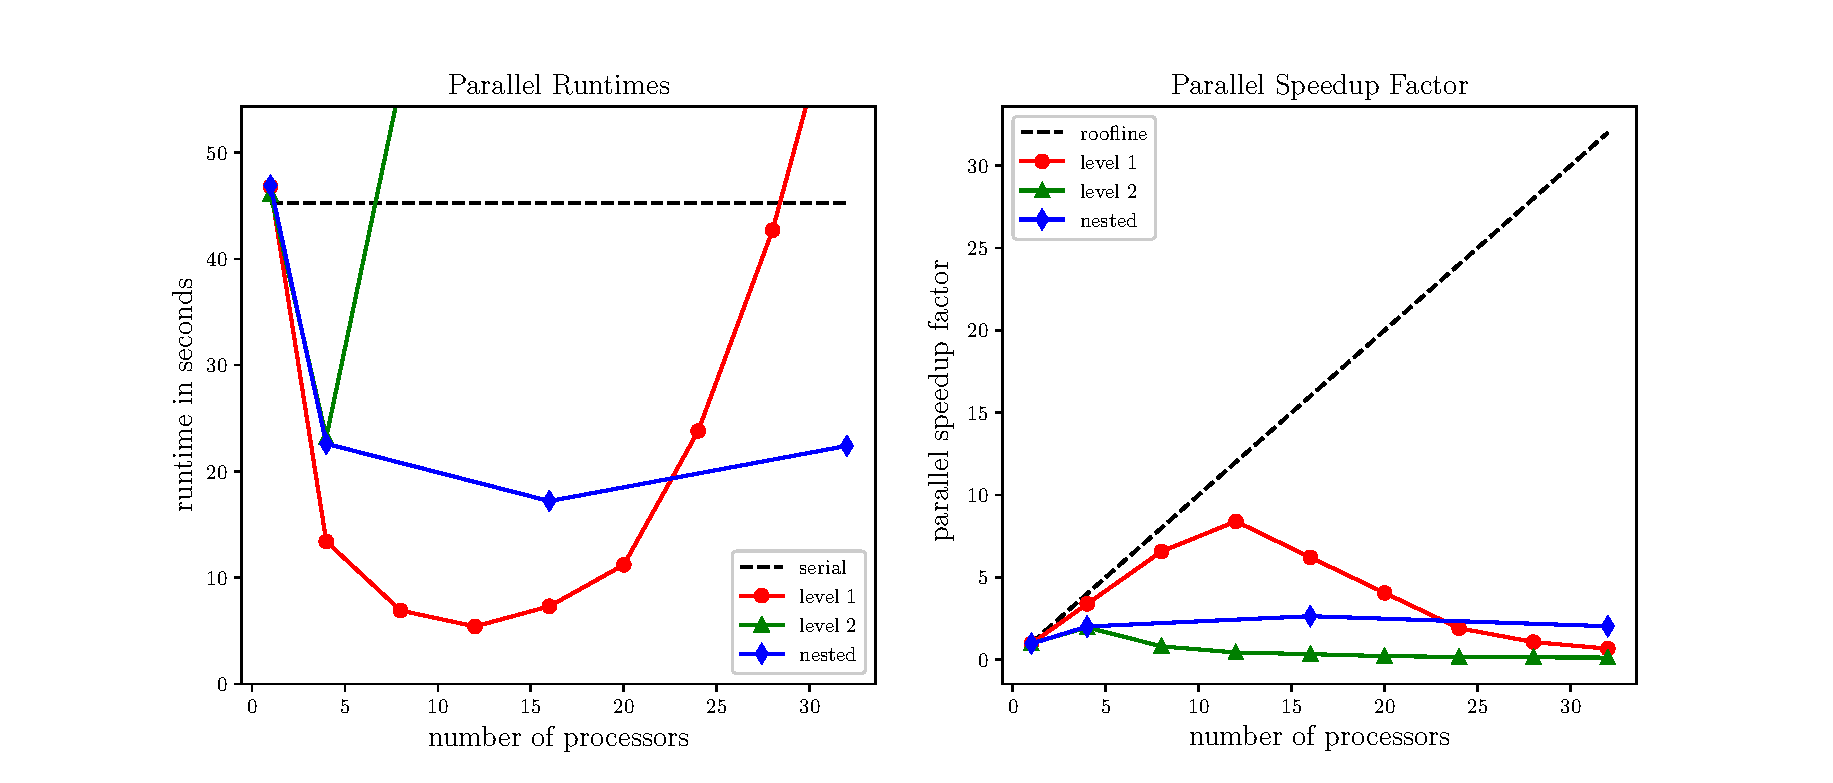
\includegraphics[width=\textwidth]{../img/delaunay_old/parallelBigM.eps}
\begin{center}$d=10\text{, }n=1000\text{, }m=1024$\end{center}
\end{column}
\end{columns}
\end{frame}

% Delaunay graph
\section{Application for Computing the Delaunay Graph}
% Introduction
\subsection{About the Delaunay Graph}
\begin{frame}{The Delaunay Graph}
\begin{itemize}
\item Delaunay graph of $P = DG(P)$
\item Connect 2 vertices iff they are shared by a single Delaunay simplex
\item Used for:
\begin{itemize}
\item Neighbor structure in spatial data
\item Topological shape analysis
\end{itemize}
\item There are at most $n(n-1)/2$ edges
\item Current state-of-the-art implementation in CGAL computes $DG(P)$ from
$DT(P)$ -- scales well for large $n$, infeasible for $d\geq10$
\end{itemize}
\end{frame}

\subsection{Algorithm using DELAUNAYSPARSE}
\begin{frame}{Getting the Delaunay Graph}
\begin{itemize}
\item The number of connections in $DG(P)$ is upper bounded by $n(n-1)/2$
\item Can recover $DG(P)$ by interpolating the midpoint between each
pair of points in $P$
\begin{itemize}
\item If the simplex containing the midpoint between $x^{(1)}$ and $x^{(2)}$
also contains both $x^{(1)}$ and $x^{(2)}$, then they are clearly connected
\item If not, then it certifies that they are not connected in {\it a}
Delaunay triangulation (in case degenerate)
\end{itemize}
\item Using {\tt DELAUNAYSPARSE}, requires
$\mathcal{O}(n^3 d^2 \ell)$ time --- better than current state-of-the-art for
$d$ large, worse for $n$ large
\end{itemize}

\medskip
Implementation currently under review for publication.

\medskip
Full proof/description in\\
{\tiny \it T.H.~Chang. Mathematical Software for Multiobjective Optimization
Problems. Ph.D.~Thesis, Virginia Tech, 2020.}
\end{frame}

\begin{frame}
  \frametitle{Questions}
  \tableofcontents
  \bigskip
{\tiny
This material is based upon work supported by the U.S. Dept.\ of Energy,
Office of Science, Office of Advanced Scientific Computing Research, SciDAC
program under contract number DE-AC02-06CH11357, and the Office of Science
Graduate Student Research (SCGSR) program.
The SCGSR program is administered by the Oak Ridge Institute for
Science and Education (ORISE), which is managed by ORAU under contract number
DE-SC0014664.
All opinions in this paper are the authors' and do not
necessarily reflect the policies and views of the DOE, ORAU, or ORISE.

This work was also supported in part by NSF Grants CNS-1565314 and CNS-1838271.
}
\end{frame}
\end{document}
